 
\section{Modules}

Modules are repositories for class lookups, and have a special entry, under \prg{Internal} to describe the internals of 

\begin{definition}[Modules]
We define modules $\syntax{Module}$ as  the set of mappings from identifiers to class descriptions or a simple assertion\\  % to force line break

\begin{tabular}  {@{}l@{\,}c@{\,}ll}
\syntax{Module} \ \  &    =   &  \ \prg{Identifier}   \     $\longrightarrow$\
$  \ ( \  \syntax{ClassDescr}     \cup  \syntax{SimpleAssertion} \ ) $
 \end{tabular}

\noindent
such that\\
 for any any $\M\in\syntax{Module}$ and the special identifier \prg{Internal} we have 
$\M(\prg{Internal})\in \syntax{SimpleAssertion}$, and for all other identifiers, \prg{C}, we have
 $\M(\prg{C})\in \syntax{ClassDescr}$ or undefined.

\end{definition}
We describe \syntax{ClassDescr}s in Definition \ref{def:syntax:classes}, and  \syntax{SimpleAssertion}s in Defintion 
??? %\ref{def:syntax:classes}.



\paragraph{Classes}

We define the syntax of class definitions below. 
Note that the language is untyped. Method bodies consist of sequences of statements; these can be field read or field assignments (only allowed if the object is \prg{this} -- i.e. as in Smalltalk), conditionals, and method calls. All else can be encoded.

 
 \begin{definition}[Classes, Methods, Args]
\label{def:syntax:classes}
We define the syntax of modules below.

\begin{tabular}{lcll}
 \syntax{ClassDescr}   &   \BBC  &     \kw{class}  \syntax{ClassId}    \lb\,  $($\ \kw{field} \syntax{FieldId}\ $)^*$ \    
 $($\ \syntax{methBody}\ $)^*$   \ \rb
\\
\syntax{methBody} &\BBC&
     \kw{method}    m\lp \syntax{ParId}$^*$ \rp   \lb\, \syntax{Stmts} \semi   \kw{return}  \syntax{Arg}  \,
    \rb
 \\
 \syntax{Stmts}  &\BBC&  \syntax{Stmt}     ~\SOR~  \syntax{Stmt} \semi \syntax{Stmts} \\
\syntax{Stmt}    &\BBC&    % \kw{var} \syntax{VarId}  {\kw{:=}} \syntax{Rhs}\\
%&  ~\SOR~ &    
 \syntax{VarId} {\kw{:=}} \syntax{Rhs}
   ~\SOR~      \kw{this}.\syntax{FieldId} {\kw{:=}} \syntax{Rhs} \\
%&  ~\SOR~ &   \kw{if}  \syntax{Arg}  \kw{then} \syntax{Stmts} \kw{else} \syntax{Stmts}\\
%&  ~\SOR~ &   \kw{skip}\\
 \syntax{Rhs} & \BBC&    {\syntax{Arg}}{\kw{.}}\syntax{MethId}\lp  \syntax{Arg}$^*$ \rp    ~\SOR~   \syntax{Arg}  
  ~\SOR~     {\kw{new} \syntax{ClassId}\lp \, \syntax{Arg}$^*$\, \rp} \\
 \syntax{Arg} &\BBC&  \syntax{ParId} ~\SOR~ \syntax{VarId} ~\SOR~ {\kw{this}} 
 % \\ &  ~\SOR~ & 
 ~\SOR~ {\kw{this}}.\syntax{FieldId}
 \end{tabular}
\end{definition}

Note that \LangOO\, supports a limited form of protection: like in Smalltalk,
  the syntax allows an object to read/write its own fields, but forbids it from reading/writing any other object's fields.
   
We define  method lookup function, $\mathcal{M}$ which returns the corresponding method definition given a class and a method identifier, where we assume that \prg{C} is a class identifier,   \prg{m} a method identifier: $ ~ $ \\

  
 \begin{definition}[Lookup]For a class identifier \prg{C}  and a method identifier \prg{m} : $ ~ $ \\

\noindent
$
\Meths {} {\prg{C}} {m}      =  \ \left\{  
\begin{array}{l}
                          \kw{method}\, m\, \lp p_1, ... p_n \rp \lb stms \semi\, \kw{return}\ {\syntax{a}} \rb\\
\hspace{1in} \mbox{if}  \M(\prg{C}) =   
\kw{class}\, \prg{C}\, \  \lb ...   \kw{method}\, m\, \lp p_1, ... p_n \rp \lb stms \semi\, \kw{return}\ {\syntax{a}} \rb  ... \rb.  
\\
\mbox{undefined},  \ \ \ \mbox{otherwise.}
\end{array}
                    \right.$
 
${\mathcal{ I}} ( {\M} ) \    =  \     \M(\prg{Internal} )$
\\

 
  \end{definition}

\subsection{The Operational Semantics of \LangOO}
\label{formal:semantics}

TODO

\subsection{Module linking}

 In this section we define  module linking and module ??? term ???
 
 Linking is an operation that takes two modules, and creates a module which corresponds  to the union of the two. We use the concept of module linking in order to model the open world, where our module $\M$ whose code we know, will be executed together with further modules whose code we do not know. 

We place some conditions for module linking to be defined: We require that the two modules do not contain implementations for the same class identifiers,  

\begin{definition}[Module Linking]

The linking operator $\circ : \syntax{Module} \times  \syntax{Module} \longrightarrow \syntax{Module}$ is defifned as follows:

$
\M \circ \M{'}  =\ \left\{
\begin{array}{l}
                        \M \circ_{aux} \M{'},\ \ \   \hbox{if}\  \ dom(\M)\!\cap\!dom(\M')\!=\!\emptyset\\
\bot  \ \ \ \mbox{otherwise.}
\end{array}
                    \right.$
                    
and where,                  
\begin{itemize}
     \item 
   For \prg{C}$\neq\prg{Internal}$, we have: \ \
   $(\M \circ_{aux} \M')(\prg{C})$ = $\M(\prg{C})$  if  $\prg{C}\in dom(\M)$, and  $\M'(\prg{C})$ otherwise.
    \item  
   $(\M \circ_{aux} \M')(\prg{Internal})$ = $ \M(\prg{Internal}) \cup  \M'(\prg{Internal})$
 \end{itemize}
\end{definition}

 
 \begin{lemma}[properties of linking]
 For any modules $\M$,   $\M'$ and $\M''$, we have$:$
 \label{lemma:linking:properties}
 
 \begin{itemize}
     \item 
     $(\M \circ \M')\circ \M''$ = $\M \circ (\M' \circ \M'')$.
    \item  
      $\M \circ \M'$  = $\M' \circ\M$.
   \end{itemize}
 
 \end{lemma}
 
\section{ Assertions}

We first define simple assertions, vvvv
 
 \subsection{Simple Assertions}
 
 \begin{definition}[Simple Expressions and simple Assertions] $ $ \\
 
 $ \SE ::=  \prg{true}  \ \mid\ \prg{false}  \ \mid \ \prg{x}  \ \mid\ \prg{this}  \ \mid \ \SE.\prg{f} \  \mid \ \SE.\prg{f} ^{k}    $

$ \SA ::= \SE  \ \mid \ \SE > \SE \ \mid \ \SA \rightarrow \SA \ \mid \ \exists x:Object.\SA  \ \mid \  \exists s:SET.\SA  \ \mid \  \exists f:FLD.\SA
 \ \mid \  \exists k:\mathbb{N}.\SA $ 

\noindent
In the above, \prg{f} is a field identifier , and  $k$ is a natural number.
\end{definition} 

The validity of simple assertions can be judged in the context of a runtime configuration

 \begin{definition}[Validity of Assertions]
We define validity of simple assertions as follows

\begin{itemize}
\item
$\sigma \models \SE$ iff $\interp{\SE}{\sigma}$ = \prg{true}.
\item
$\sigma \models \SEOne>\SETwo$ iff $\interp{\SEOne}{\sigma}$ > $\interp{\SETwo}{\sigma}$
\item
...
\end{itemize}
\end{definition}

Simple assertions form a classical logic: TODO: check the term; also to check whether we need any more from the classical logic's properties, since the rest of them probably hold by definition.

\begin{lemma}[Simple Assertions are classical]
For all runtime configurations $\sigma$, and simple assertions $\SA$, we have
\begin{itemize}
\item
$\sigma \models \SA$ or $\sigma \models \neg\SA$
\end{itemize}
\end{lemma}
\begin{proof} By induction over the structure of $\SA$. \end{proof}.
 
 \subsection{Assertions}

We now define an "full assertions" ....

We will define the OCAP assertions $\CanAccess{\_}{\_}$  (permission)
and   $\Changes{\_}$ (authority). \footnote{Note that they are slightly different
assertions to those we had in the past.}
We also add temporal modifiers, where $\Future \A$ expresses that $\A$ will hold at some future point,
$\Past \A$ expresses that $\A$ held at some point in the past.
We also add a {\em spatial modifier}, $\Using{\A}{S}$, which expresses that assertion $\A$ holds in
the sub-configurations determined by the witness \prg{S}.

We extend the syntax for assertions as follows:\footnote{The symbols are not that good -- esp the symbols for future and past.}

\begin{definition}[Assertions]
$$\A ::=\  ... \mbox{as before} ...\ \ \mid \ \CanAccess x y \ \mid\  \ \Changes e \ \mid\  \Calls{m} \ \mid\  \\ \Future \A \ \mid \ \Using \A S  \ \mid \  \Past \A$$
\end{definition}

\end{document}

\begin{definition}[Time, Permission, Authority,  and Space ]
\label{def:permission}
Given a module $\M$, identifiers \code{x} and \code{y}, expression $\sE$, and runtime configuration $\sigma$, and a set of addresses $S$,
we define validity of the assertions   .... as follows:

\begin{itemize}
\item
$\Prog{},\sigma \models  \Future \A$\ \ iff\ \  $\exists \sigma'.\, [\ \ \M,\sigma \leadsto^* \sigma' \ \wedge \ \M,\sigma' [\overline{x \mapsto \sigma(x)}]\models \A, \mbox{ where } \overline{x}=Free(\A)\   ]$.
\item
$\Prog{},\sigma \models  \Past \A$\ \   iff\ \  $\exists \sigma_1,....\sigma_n, k\!\in\![1..n-1).\ [ \Initial {\sigma_1}\  \wedge\ \sigma_n=\sigma\ \wedge\ \forall i\!\in\![1..n).\ \M,\sigma_i\leadsto  \sigma_{i+1}  $\\
\strut \hspace{5.7cm} $\ \wedge \  \ \M,\sigma_k[\overline{x \mapsto \sigma(x)}]\models \A, \mbox{ where } \overline{x}=Free(\A)\  ]$.
\item
$\Prog{},\sigma \models   \CanAccess{\prg{x}}{\prg{y}}$   \ \ iff  \begin{itemize}
\item
$\sigma(x)$=$\sigma(y)$, or
\item
$\sigma(\prg{x},\prg{f})$=$\sigma(\prg{y})$  for some field \prg{f},  or
\item
$\sigma(\prg{this})$=$\sigma(\prg{x})$ and
  $\sigma(\prg{z})$=$\sigma(\prg{y})$,
  $\strut \hspace{0.1cm}$
for some some parameter of local variable \prg{z}.
 \end{itemize}
 \item
 $\Prog{},\sigma \models   \Changes{\prg{e}}$   \ \ iff \  \
 $\exists \sigma'.\, [\ \ \M,\sigma \leadsto \sigma' \ \wedge \interp{e}{\M,\sigma} \neq \interp{e}{\M,\sigma'}\ \ ]$


\item
 $\sigma\!\mid_S$ denotes a {\em restriction} of $\sigma$ to the objects from the set $S$. That is, the domain of
 the heap in $\sigma\mid_S$ is $S$, and otherwise,  $\sigma\mid_S$ is identical to $\sigma$. An example appears in figure \ref{fig:DiagramRestricted}.
 \item
$\M,\sigma  \models \Using{\A}{\prg{S}}$  \  \ iff \ \
  $ \M,\sigma\!\mid_S\, \models \A $, where   $S=\interp {\prg{S}} {\M,\sigma} $.
 \item
 $\M,\sigma  \models \Calls {m}$ \ \ iff \ \ the method call in the current frame in $\sigma$ is
 \prg{m}\footnote{We will express this precisely  when we have the full definition of $\sigma$}
\end{itemize}
\end{definition}

\begin{figure}[btph]
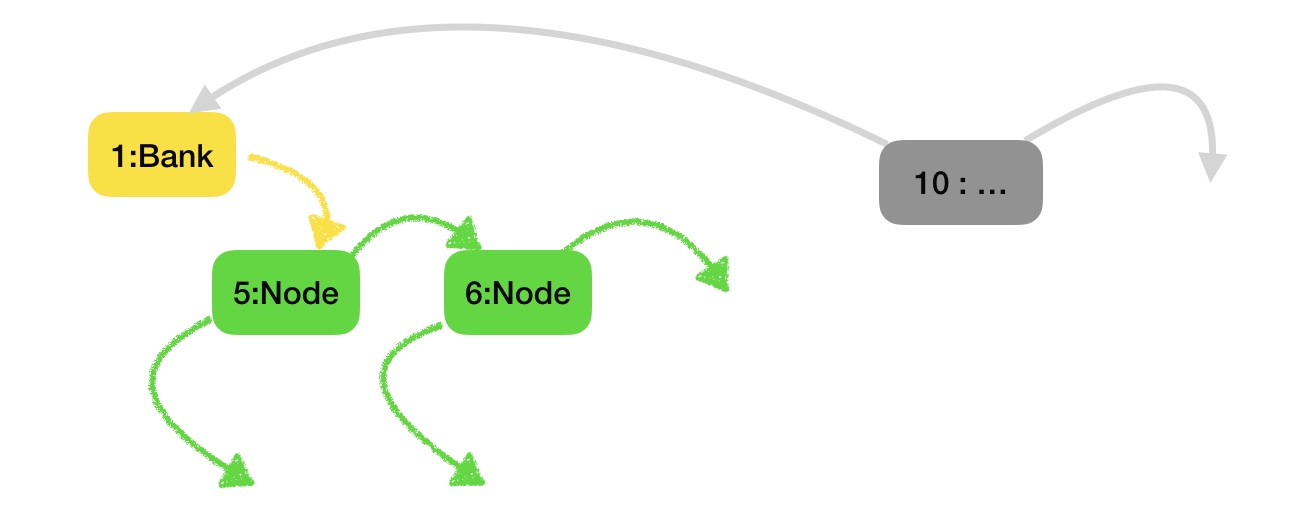
\includegraphics[width=10cm,height=4cm]{diagram2}
 \caption{Configuration from Fig. \ref{fig:Diagram} restricted to witness \{ \prg{1}, \prg{5}, \prg{6}, \prg{10} \}}
  \label{fig:DiagramRestricted}
  \end{figure}

Note that $\CanAccess{\prg{x}}{\prg{y}}$ is reflexive but  not transitive and not symmetric.

Also note the difference between $\Using{(\Future{\A})}{\prg{S}}$ and $\Future{(\Using{\A} }{\prg{S}})$.
For example,  the assertion  $\Using{(\Future{\prg{x}.\prg{f}=\prg{z}})}{\prg{S}}$ expresses that the current execution
leads to a future configuration  where
$\prg{x}.\prg{f}=\prg{z}$ will hold, and that the set \prg{S} suffices to witness this execution, while the assertion
$\Future{(\Using{{\prg{x}.\prg{f}=\prg{z}} }}{\prg{S}})$  expresses that the current execution
leads to a future configuration   where
$\prg{x}.\prg{f}=\prg{z}$ will hold and where  the set \prg{S} suffices to witness
that fact.
For example, take a configuration $\sigma$ where variable \prg{x} maps to some object \prg{31}, and where \prg{31} has a field \prg{f}
pointing to \prg{32}, and \prg{32} has a field \prg{f}
pointing to \prg{33}, and variable \prg{z} maps to  \prg{33}. Assume also that the expression to be executed in $\sigma$ starts with
\prg{x.f}=\prg{x.f.f}. Then we have that
$\M,\sigma  \models \Future{(\Using{{\prg{x}.\prg{f}=\prg{z}} }{\{\prg{x},\prg{z}\}})}$,
but
$\M,\sigma  \not\models \Using{(\Future{\prg{x}.\prg{f}=\prg{z}})}{\{\prg{x},\prg{z}\}}$.
On the other hand
$\M,\sigma  \not\models \Using{(\Future{\prg{x}.\prg{f}=\prg{z}})}{\{\prg{x},\prg{x}.\prg{f},\prg{z}\}}$

In general, for all $\M$ and $\sigma$, we have that
 $\M,\sigma \models  \Using{(\Future{\A})}{\prg{S}}$ implies $\M,\sigma \models \Future{(\Using{\A} }{\prg{S}})$, and that
 $\M,\sigma \models \Future{(\Using{\A} }{\prg{S}})$ implies that there exists a set $\prg{S}'$ such that
 $\M,\sigma \models  \Using{(\Future{\A})}{(\prg{S}\cup\prg{S'})}$.

\vspace{.2in}
We will prove that

\begin{lemma}[Preservation of validity and module linking]

$\M,\sigma \models \A$  \ \ \ then\ \ \ \   for all $\M'$ with $\M*\M'$ is defined:\ $\M*\M',\sigma \models \A$.
\end{lemma}




\subsection{Invariants}

We define below the meaning of invariants.\footnote{This part is as we had defined previously, with two simplifications: a) we do not need to worry about the $\obeys$-predicate here, and b) we do not distinguish the names of the classes and the names of participants in interfaces.}
The assertion $\M   \models\  \A$ requires that  the assertion $A$ is satisfied
in all reachable states.

\begin{definition}[Invariants]
\label{def:invariant}
\noindent
For a module $\M$  and assertion $\A$ we define:\\

 \begin{itemize}
 \item
$\M   \models\  \A$\ \ \  iff\ \ \ \
% $\strut\SP\SP$
$\forall \M'.\, \forall \sigma\!\in\!\Arising(\M'*\M).\ \M'*\M,\sigma \models \  \A$
 \end{itemize}
\end{definition}

The use of the set of configurations from $\Arising(\M'*\M)$ reflects that policies
 need to hold in an {\em open} world, where
we link against {\em any} module $\M'$,
about which we know nothing.

\subsection{Implication and equivalence}

\begin{definition}
\label{def:impl:equiv}
\noindent
For a module $\M$  and assertions $\A$  and $\A'$, we define strong equivalence and implication ($\equiv$ and $\sqsubseteq$), as well
as   weak equivalence and implication ($\approxeq$ and $\weakImplies$)  as follows:


 \begin{itemize}
\item
$\M   \models\  \A \strongImplies \A'$  \ \ \ \ iff \ \ \ \
$\forall \M'.\, \forall \sigma\!\in\!\Arising(\M'*\M).[\ \ \  \M'*\M, \sigma \models \A \  \ \  \longrightarrow\  \ \  \M'*\M, \sigma \models \A'\ \ \ ]$
 \item
$\M   \models\  \A \equiv \A'$ \ \ \ \ iff \ \ \ \
$\M   \models\  \A \strongImplies \A'\ \  \wedge \ \  \M   \models\  \A' \strongImplies \A$
%$\forall \M'.\, \forall \sigma\!\in\!\Arising(\M'*\M):\ \ \  \M'*\M, \sigma \models \A \  \ \longleftrightarrow\   \ \M'*\M, \sigma \models \A'$
\item
$\M   \models\   \A \weakImplies \A'$  \ \ \ \ iff \\ \ \ \ \ \ \
\strut  \hspace{1cm}  $\forall \M'.\, \forall \sigma\!\in\!\Arising(\M'*\M).\,\M'*\M, \sigma \models \A$ \  \ \  $\longrightarrow$\  \ \
$\forall \M'.\, \forall \sigma\!\in\!\Arising(\M'*\M).\,\M'*\M, \sigma \models \A'$
\item
$\M   \models\  \A \approxeq \A'$   \ \ \ \ iff \ \ \ \ \
$ \M  \models  \A \weakImplies \A' \   \ \wedge\   \  \M  \models  \A' \weakImplies \A$
 \end{itemize}
\end{definition}

The definitions from above are applicable to the empty module, eg  $\models\  \A \equiv \A'$ iff   all modules $\M$ satisfy $\M \models\  \A \equiv \A'$.
The following properties hold:

\begin{lemma}
For all modules \M, assertions \A and \A':

 \begin{itemize}
 \item
$\M   \models\  \A \equiv \A'$  \ \ \ implies \ \ \  $\M   \models\  \A \simeq \A'$
\item
$\M   \models\  \A \strongImplies \A'$  \ \ \ \ implies  \ \ \ \
$\M \models \A \weakImplies \A$
\item
$\M \models   \Using{(\Future{\A})}{\prg{S}}\ \strongImplies\ \Future{(\Using{\A} }{\prg{S}})$
\item
$ \M \models\  \Future{\A}\rightarrow \A' \  \  \weakImplies \ \ \A\rightarrow\Past{\A'}$
 \end{itemize}
\end{lemma}

\paragraph{Space-Monotonicity}\footnote{Not sure how useful this concept is}

\begin{definition}[Space-Monotonicity]
We call an assertion $\A$ {\em space-monotonic} in $\M$, iff for all set expressions $\prg{S}$ and  $\prg{S}'$,
  % $\M,\sigma\models ( \prg{S} \subseteq \prg{S}'\ \wedge\  \Using{\A, \prg{S}}) \ \strongImplies\  (\Using{\A, \prg{S'}})$
%\end{definition}\footnote{If we unfold the definitions, we obtain that
% $\A$ is space-monotonic in $\M$, iff for all set expressions $\prg{S}$ and  $\prg{S}'$
 and all $\sigma\in\Arising({\M})$:
 \\
  If  $\M,\sigma\models  \prg{S} \subseteq \prg{S}'$ and $\M,\sigma\models  \Using{\A} {\prg{S}}$, then
$\M,\sigma\models  \Using{\A}{ \prg{S'}}$
\end{definition}

We prove space monotonicity for some assertions

\begin{lemma}[Space-Monotonicity for change and access]
$ ~ $

\begin{itemize}
\item
${\Changes \sE} $ is space-monotonic.
\item
$\CanAccess {\prg{x}}{\prg{y}}$ is space-monotonic.

\end{itemize}
\end{lemma}

Not all assertions  are not space-monotonic. E.g. $\forall a:\prg{Account}.\prg{a.balance}\geq 3$ is not space-monotonic.


The following lemma would be nice to have -- otherwise we will need to change the definition of monotonicity.

\begin{lemma}[Space-Monotonicity and module linking]
If $\A$ is space-monotonic with $\M$, then it is also space-monotonic with $\M*\M'$.
\end{lemma}


 \section{Specifications for Robustness Policies}

 We now use the concepts introduced in the earlier sections to specify various robustness policies

 \subsection{Specification of \Pol 2  and   \Pol 4}

We    give a formal definition of \Pol 2 and  \Pol 4, using the concepts defined earlier in  Definition \ref{def:permission}: %

\begin{definition}
\label{def:pol2}
We define  what it means for an object \prg{o} to be internal to a bank's data structure, an then define \Pol 2  and   \Pol 4  as follows:

%  \noindent
$\prg{Internal}(\prg{b})$ \ \  $\triangleq$ \ \
$\{\ \prg{o}\ \mid\  \prg{b}:\prg{Bank}\ \ \wedge \ \ (\ \prg{o} = \prg{b}\ \ \vee\  \ \prg{o}:\prg{Account}\wedge \prg{o}.\prg{myBank}=\prg{b}$\\
\strut \hspace{7.3cm} $\ \ \vee\ \ \ \exists k. \ \prg{b}.\prg{ledger}.\prg{next}^k = \prg{b})\ \ \ \ \}$


$\prg{Internal}'(\prg{a})$ \ \  $\triangleq$ \ \
$\{\ \prg{o}\ \mid\  \prg{a}:\prg{Account}\ \ \wedge \ \
 \prg{a}.\prg{myBank} :\prg{Bank}\ \wedge\  \prg{o}\in \prg{Internal}(\prg{b})\ \}$


 \vspace{.2cm}

  \Pol 2\ \  $\triangleq$ \ \
  $\forall \prg{b}.\forall \prg{S}.
  [ \ \  \prg{b}:
  \prg{Bank}\ \wedge\ \prg{this}\neq\prg{b}\ \wedge\ \ \Using{(\Future\Changes{\prg{b.currency}})}{\prg{S}} \ \ \ \ \longrightarrow \ \  $\\
   \strut $~ $ \ \ \ \hspace{1.7in}  \hfill
 $\exists \prg{o}. \ [ \ \
  \prg{o}\in \prg{S}\   \wedge\  \CanAccess{\prg{o}}{\prg{b}}\ \wedge\     \prg{o}\notin\prg{Internal}(\prg{b})  \ \ ]\ \ ]$


 \vspace{.1cm}
% \noindent
    \Pol 4\ \  $\triangleq$\ \ $\forall \prg{a}.\forall \prg{S}.\ [ \ \  \prg{a}:\prg{Account}\   \wedge\   \prg{this}\neq\prg{a} \ \wedge\ \Using{(\Future\Changes{\prg{a.balance}})}{\prg{S}}\ \ \   \
    \longrightarrow$ \\
 $\strut \hspace{3.9cm} \hfill \exists \prg{o}.\ [\, \prg{o}\in \prg{S}\ \wedge \ \CanAccess{\prg{o}}{\prg{a}}\ \wedge  \ \prg{o} \notin\prg{Internal}'(\prg{a}) \ ] \ \ \ \ ]$

\end{definition}

\paragraph{Discussion}
In other words, \Pol 2  mandates that the elements of the data structure (ie the elements from $\prg{Internal}(\prg{b})$) cannot be used (are not sufficient) to  change the currency of the bank. If a computation takes place inside the set \prg{S}, and {\em in the current state} in \prg{S}
all accesses to the bank go through elements of the data structure (ie the \prg{Account} objects),\footnote{Say why we can ignore \prg{Node} objects} then we have a guarantee that the computation will not affect the currency.
For example, if a computation takes place in the context of objects \prg{1}, \prg{2}, \prg{3}, \prg{4}, \prg{5}, \prg{7}, \prg{20} and \prg{21}, and the current receiver is no \prg{1}, then we have a guarantee that the currency of \prg{1} will not be affected. So, even through \prg{1} is involved in the computation, because there is no {\em external} access to it, we have a guaratee that the method \prg{makeAccount} will not be called on it.

An alternative way of expressing \Pol 2 is as follows:


 \Pol 2\ \  $\equiv$ \ \
  $\forall \prg{b}.\forall \prg{S}.
  [ \ \  \prg{b}:
  \prg{Bank}\ \wedge\   \prg{b}\neq\prg{this}\ \wedge\  \forall \prg{o} \in \prg{S}.\, [\ \prg{o}\in\prg{Internal}(\prg{b}) \ \vee\  \neg  \CanAccess{\prg{o}}{\prg{a}}  \ \ ]$
\\ \hfill \strut $~   \ \ \ \hspace{1.7in}  \  \ \longrightarrow \ \ \ \neg(
 \Using{(\Future\Changes{\prg{b.currency}})}{\prg{S}})\   \  \ \ ]$

\vspace{.01in}
% TO\_DO: discuss the difference between  $\Using{(\Future\Changes{\prg{b.currency}})}{\prg{S}})$, and
% $\Future{(\Using{\Changes{\prg{b.currency}}{\prg{S}})}}$.

\vspace{.01in}
\Pol 2  guarantees
that if an object \prg{o}$\neq$\prg{b} may affect the value of \prg{b.Currency} only if the  objects
involved in the process of affecting the value of \prg{b.Currency}  include at least an object $\prg{o}'$
which had direct access to \prg{b}, and
whose class is  not  \prg{Account}. Stated positively, this policy mandates
that exporting an \prg{Account} to an environment will not affect the \prg{Currency} of \prg{b}.
In other words,
\prg{Account}s protect the integrity of the \prg{Bank}'s currency.


In more detail, by applying  Definition \ref{def:invariant} on Definition \ref{def:pol2}, the  meaning of policy \Pol 2
  is, that a runtime configuration $\sigma$ satisfies  \Pol 2  if whenever the current receiver in $\sigma$
 is not a \prg{Bank} object, and the execution of $\sigma$ leads to another runtime configuration $\sigma'$
 with a different value for \prg{b.Currency}, then the objects involved in the execution from
 $\sigma$ to $\sigma'$ include at least one object which had direct access to \prg{b}.
 Note that this direct access needs to exist at the beginning of   the execution, \ie at $\sigma$.
 Formally:

 \noindent
 $\M, \sigma \models  \Pol 2$\\$ \strut \ \ \ \  \ \  \longleftrightarrow $\\
 $\forall \prg{b}.\forall S.\ [ \ \ \ \ \M, \sigma \models \prg{b}:\prg{Bank}\ \wedge\
 \sigma(\prg{b})\neq \ \sigma(\prg{this}) $\\
 $\strut \hspace{2.1cm}  \wedge \
 \ \exists\sigma'.(\ \ \ \ \M, \sigma\mid_S \leadsto^* \sigma'\
\ \wedge\ \interp {\prg{b.Currency}}{\M,\sigma}\neq \interp {\prg{b.Currency}}{\M,\sigma'[\prg{b}\mapsto\sigma(\prg{b})]}\ )$\\
$\strut \hspace{4.7cm} \longrightarrow$ \\
 $\strut \hspace{2.7cm}  %\exists \prg{o}. (\ \  \sigma(\prg{o}) \!\!\in\!\!\prg{S}\ \
 \exists \prg{o}. (\ \ \prg{o} \!\in\!S\ \
  \wedge \ \ \M, \sigma \models \CanAccess{\prg{o}}{\prg{b} }\ \wedge \  \prg{o}\notin \prg{Internal}(\prg{b}) \   \ ) \ \ \ \ \ \ \  ]$



\subsection{Specifying  "no leaks"}

This is a family of guarantees that Dean seemed especially interested in, when we discussed in March in London.
For the particular example, we want to express that

\begin{description}
\item[\Pol 7]
The \prg{Bank} does not leak out of the \prg{Bank}/\prg{Account} system
%\item[Pol\_7]
%The \prg{Accounts} do  not leak out of the \prg{Bank}/\prg{Account} system
\end{description}

And we give a formal specification

\begin{definition}[Banks do not leak]
\label{def:bankNoLEak} We define \Pol 7 as follows:

\Pol{7}\ \  $\triangleq$\ \ $\forall \prg{b}.\forall \prg{S}.\ [  \ \ \prg{b}:\prg{Bank}\ \wedge\  \prg{o}:\prg{Object}\  \wedge\   \neg(\CanAccess{\prg{o}}{ \prg{b}})\ \wedge\   \Using {(\Future{\CanAccess {\prg{o}}{\prg{b}}})} {\prg{S}} $
 \\  $\strut$ \hspace{4cm}
  $\longrightarrow$
 $\strut \hspace{0.5cm}  \exists \prg{o}'.\ [\, \prg{o}'\in \prg{S}\ \wedge \  \CanAccess{\prg{o}'}{ \prg{b} }\ \wedge\   \prg{o}' \notin \prg{Internal}(\prg{b}) \, ) \ ] \  \  \ \  ]$

%\hspace{.1cm}
%{\bf {Pol\_8}}\ \  $\equiv$\ \ $\forall \prg{o},\prg{b}, \prg{o}'\forall \prg{S}.\ [  \ \ \prg{b}:\prg{Bank}\ \wedge \prg{o}\in\prg{Internal}({\prg{b}})\ \wedge\  \prg{o}':\prg{Object}\ \ \neg(\CanAccess{\prg{o}'}{ \prg{o}})\ \wedge\   \Using {(\Future{\CanAccess {\prg{o}'}{\prg{o}}})} {\prg{S}} $
% \\  $\strut$ \hspace{4cm}
%  $\longrightarrow$
% $\strut \hspace{0.5cm}  \exists \prg{o}''.\ [\, \prg{o}''\in \prg{S}\ \wedge \  \CanAccess{\prg{o}''}{ \prg{o} }\ \wedge\   \prg{o}'' \notin \prg{Internal}(\prg{b}) \, ) \ ] \  \  \ \  ]$
\end{definition}

In other words, \Pol 7 guarantees that objects that are internal to the bank \prg{b} do not leak access to it.
In more detail: if   objects  \prg{o} and \prg{b} exist  now, and \prg{o} does not have direct access to \prg{b} now, but obtains
access to \prg{b} through some computation which involves objects from the set \prg{S}, then at least one  object  from \prg{S} has
now direct access to   \prg{b} and this object is not internal to \prg{b}.

\section{Adherence to Policies}
\label{section:Adherence}
In this section we will outline the proofs that particular modules adhere to their specifications.
This serves to demonstrate the practicality of our approach.
In particular we will show two different versions fo the \prg{Bank}/\prg{Account} example (sections \ref{section:Adherence:ModuleOne} and \ref{section:Adherence:ModuleTwo}, and we will prove that
both satisfy the policies \Pol 2, \Pol 4, and \Pol 7, while they differ in the definition of \prg{Internal}.
But before doing that, in section \ref{section:GeneralPropertiesExecution}, we will study some further properties of execution.


\subsection{General properties of execution}\footnote{Find better title?}
\label{section:GeneralPropertiesExecution}

We will first define some further predicates which reflect over the program execution and prove
some general properties of program execution.

We call a locations set, \prg{L}, an expression which denotes a set of addresses and field identifiers, \eg, $\{\ (\prg{b},\prg{ledger}), (\prg{b}.\prg{ledger},\prg{balance})\ \}$ is such a locations set.

\begin{definition}[Framing]
Take arbitrary module \M, assertion \A, , ...

\begin{itemize}
\item
\interp{\prg{L}}{\sigma,\M*\M'} = ....
\item
$ \sigma\mid _L$ ....
\item
$\M, \sigma \models \prg{L} \frames \prg{e}$\ \ \ \  \ iff \ \ \ \ \
$\forall \M'.\forall \sigma'\!\in\!\Arising({\M*\M'}). \forall L.$\\
\strut \hspace{1cm} $  [ \ \ L=\interp{\prg{L}}{\M,\sigma}\, \wedge\,
 \sigma\mid _L= \sigma'\mid_L \ \   \longrightarrow\ \ \   \interp {\prg{e}}{\sigma,\M*\M'}  =  \interp {\prg{e}}{\sigma',\M*\M'}
\ \ ]$
\item
$\M  \models \prg{L} \frames \prg{e}$\ \ \ \  \ iff \ \ \ \ \
$\forall \M'.\forall \sigma\!\in\!\Arising({\M*\M'}). \ \M'*\M, \sigma \models \prg{L} \frames \prg{e}$
\item
$\M, \sigma \models \prg{L} \frames\A $\ \ \ \  \ iff \ \ \ \ \
$\forall \M'.\forall \sigma'\!\in\!\Arising({\M*\M'}). \forall L.$\\
\strut \hspace{1cm} $ [ \ \ L=\interp{\prg{L}}{\M,\sigma}\, \wedge\,
\sigma\mid _L= \sigma'\mid_L \ \   \longrightarrow\ \ \   [\ \M*\M',\sigma \models \A   \ \longleftrightarrow\ \M*\M',\sigma' \models \A
\ \ ] $
\item
$\M  \models \prg{L} \frames \A$\ \ \ \  \ iff \ \ \ \ \
$\forall \M'.\forall \sigma\!\in\!\Arising({\M*\M'}). \ \M'*\M, \sigma \models \prg{L} \frames \A$
\end{itemize}

\end{definition}

NOTE\_TO\_SELF: we need to think about whether we also need to make \prg{L} self-framing.
Also, rethink whether we need to stick new modules $\M'$ to the whole thing.
--
Also, the sets are not equal -- they are isomorphic. We can deal with isomorphisms, but
it has a high notation penalty. Can we pretend that they are equal? hmhhhhh


And then we can prove that changes in the interpretation or the validity require a change in the frame:

\begin{lemma}[Change in the context of framing]
Take arbitrary module \M, assertion \A, such that  $\sigma\in\Arising({\M*\M'})$

\begin{itemize}
\item
If  $\M  \models \prg{L} \frames \prg{e}$, and
$\M'*\M, \sigma \models \Using{(\Future{\Changes{\prg{e}}})}{\prg{S}}$, \\
then there exists a pair $(\prg{e}',\prg{f})$ , with
$\M,\sigma \models (\prg{e}',\prg{f})\in \prg{L}$\footnote{Sophia, you need to check this bit  what if \prg{z}
there is no handle in \prg{L}, eg what if \prg{L} talks about anonymous objects
\eg \prg{L} = $\{ o \ \mid o.\prg{myBank}=\prg{b} \}$?Here $o$ is anonymous. Also, do we need $\M$ or $\M'*\M$?}
and $\M'*\M, \sigma \models  \Using{\Future{\Changes{\prg{e}'.\prg{f}}}}{\prg{S}}$

\item
similar for
$\M'*\M, \sigma \models \Using{\Future{\Changes{\A}}}{\prg{S}}$
\end{itemize}

\end{lemma}

\begin{figure}[tbp]
\begin{lstlisting}
 class Bank {
   private field ledger;   // a Node

   Bank( )
     { ledger = null; }
   fun makeAccount(amt)
     { account = new Account(this);
       ledger = new Node(account, amt, ledger);
       return account; }
   fun deposit(source, destination, amnt)
     { sourceNd = ledger.getNode(source)
       destinationNd = ledger.getNode(destination)
       if (sourceNd!=null && destinationNd!=null && sourceNd.balance>amt) then
          { < sourceNd.balance = sourceNd.balance-amt
              destinationNd.balance = destinationNd.balance+amt > }
        else
          { return }               }
 }

 class Account {
   private field myBank;  // a Bank

   Account(aBank)
     { myBank = aBank;  }
   fun sprout( )
     // create Account in same Bank with 0 balance
     { return this.myBank.makeAccount(0)  }
   fun deposit(source, amnt)
     // if destination is an Account in myBank,  and  source holds enough money,
     // then transfer amnt from source into receiver
     { myBank.deposit(source,this,amnt) }
 }

  class Node{
   field balance;     // the  money held in theAccount a number
   field next;        // the next node
   field theAccount;  // the account

   fun getNode(account)
     { if (theAccount==account) then
           { return this }
       elseif (next!=null)
           { next.getNode(account) }
       else
           {  return null }            }	
 }
\end{lstlisting}
\caption{\MOne: First version of the Bank example, in detail}
\label{fig:BankDetailedOne}
 \end{figure}


We now think a bit more about changes in accessibility. The predicate  $\Gives(\prg{x},\prg{y},\prg{z})$ expresses
that \prg{x} passed to \prg{y} access to \prg{z}.

\begin{definition}[Giving]
For arbitrary module \M and $\sigma$, we define:

\begin{itemize}
\item
$\M,\sigma  \models \Gives(\prg{x},\prg{y},\prg{z})$\ \ iff \ \
$\sigma(\prg{this})$=$\sigma(\prg{x})$ \  $\wedge$ \
$\M, \sigma \models \neg (\MayAccess( \prg{y},\prg{z})\,)$ \ $\wedge$ \\
\strut \hspace{.9cm} $\exists \sigma'. \ [\  \M,\sigma \leadsto \sigma'  \  \wedge  \
 \M,\sigma' \models \MayAccess( \prg{y},\prg{z})\ ]$
\end{itemize}

\end{definition}

The following lemma says that any changes in accessibility witnessed\footnote{is that the right term? or frames?}
by set \prg{S} is due to an element of \prg{S} giving the object.

\begin{lemma}[Change in Accessibility is caused by Giving]
For any module \M, and  $\sigma$

\begin{itemize}
\item
If  $\M, \sigma  \models \neg(\MayAccess(\prg{y},\prg{z}))$, and
$\M, \sigma \models \Using{(\Future \MayAccess(\prg{y},\prg{z}))}{\prg{S}}$, \\
 then there exists a  $\prg{x}$  and  $\prg{y}'$, with
%$\M,\sigma \models  \prg{e} \in \prg{S}$, and
$\M,\sigma \models \Using{(\Future{\Gives(\prg{x},\prg{y}',\prg{z})})}{\prg{S}}$.
\end{itemize}

\end{lemma}

\subsection{Adherence to Policies for module \MOne}
\label{section:Adherence:ModuleOne}

In figure \ref{fig:BankDetailedOne} we show the  code for \MOne in detail.

\subsubsection{\MOne~preliminaries}
We define the footprint of \prg{b.balance} as

\begin{definition}We define the currency-footprint of a bank as follows:

$\prg{CurrencyFootprint}(\prg{b})$ $\triangleq$
$\{ \ (\prg{b},\prg{ledger}) \} \ \cup$\\
\strut \hspace{4.8cm}
$\{ \ (\prg{o},\prg{balance})\ \mid \exists k:\mathbb{N}. \prg{x}.\prg{ledger}.\prg{next}^k=\prg{o} \ \}$
\end{definition}

\begin{lemma}
$\MOne \models \prg{b}:\prg{Bank} \rightarrow \prg{CurrencyFootprint}(\prg{b}) \frames \prg{b}.\prg{currency}$
\end{lemma}

We also define a predicate $Gives(prg{x},prg{y},prg{z})$ which expresses that while \prg{x} was excuting, it
passed to \prg{y} access to \prg{z}.
... more in handwritten notes ...

\subsubsection{\MOne~adheres to \Pol 2}
\begin{lemma}
$\MOne \models \Pol 2$
\end{lemma}
Proof sketch   in Sophia's handwritten notes.

\subsubsection{\MOne~adheres to \Pol 4}

\begin{lemma}
$\MOne \models \Pol 4$
\end{lemma}

\subsubsection{\MOne~adheres to \Pol 7}

\begin{lemma}
$\MOne \models \Pol 7$
\end{lemma}
Proof sketch  in Toby's handwritten notes.

\subsection{Adherence to Policies for module \MTwo}
\label{section:Adherence:ModuleTwo}

In figure \ref{fig:BankDetailedTwo} we show the  code for \MTwo in detail.

\begin{figure}[tbp]
\begin{lstlisting}
 class Bank {    }

 class Account {
   protected field balance; // the data of the Account;
   protected field myBank;  // a Bank

   Account(aBank,amt){
     balance = amt;
     myBank = aBank }

   fun deposit(source, amnt){
     if ( myBank== source.myBank && source.balance>=amt && amt>0) then
        { source.balance = source.balance-amt;
           this.balance = this.balance + amt }    }
}

\end{lstlisting}
\caption{\MTwo: Second version of the Bank example, in detail}
\label{fig:BankDetailedTwo}
 \end{figure}

We give the code for \MTwo~ in Figure ???, and define \prg{Internal} as follows.
The code works through ...
The set  \prg{Internal} describes ....


\subsubsection{\MTwo~adheres to \Pol 2}

\subsubsection{\MTwo~adheres to \Pol 4}

\subsubsection{\MTwo~adheres to \Pol 7}


\section{Hoare Logic}
\label{section:Hoare}
Here we give Hoare Logic rules which allow us to prove adherence to policies.
NOTE: Not sure when we will get to do these rules. If we get to define these rules, then we will use them for the proofs
 in section \ref{section:Adherence:ModuleOne}
and we will swap section \ref{section:Adherence} and section \ref{section:Hoare}

\section{Further Applications}
In this section we will apply our methodology to give specifications to other famous patterns from the OCAP literature,
\ie the membrane, the DOC-tree, and ...

\subsection{The DOM tree}
....

\subsection{The membrane}
...

\subsection{Sealer/Unsealer}

In Figure \ref{fig:WrapUnwrap} we visit the sealer/unsealer example  from cite-Morrison and Miller.


\begin{figure}[tbp]
\begin{lstlisting}
 class Box{
   ...
   fun seal(element){... }
   fun unseal(sealed){ ... }
 }

\end{lstlisting}
\caption{Wrapping and Unwrappingl}
\label{fig:WrapUnwrap}
 \end{figure}

The specification of these functions mandates \prg{seal} wraps the object into another structure, and \prg{unseal} unwraps the original object out of the structure, Like cite(David Swasey, OOPLSA'13), we use an uninterpreted  predixate, $\prg{Wrapped}(\prg{z},\prg{o},\prg{b})$ which expresses that \prg{z} contains the value of \prg{o} as wrapped by \prg{b}.

The policies from below express that \prg{seal} wraps an object, while \prg{unseal} unwraps it, and they are very similar to those from cite(David Swasey, OOPLSA'13).

\Pol {seal\_1} $\triangleq$
\strut \hspace{2.1cm} $\prg{o}:\prg{Object}\ \wedge\ \prg{b}:\prg{Box}$  \\
\strut \hspace{6cm}$\{\ \prg{x} = \prg{b}.\prg{seal}\prg{(o)}\ \}$\\
\strut \hspace{5cm} $\prg{Wrapped}(\prg{x},\prg{o},\prg{b})$

\hspace{.1cm}

\Pol {seal\_2} $\triangleq$
\strut \hspace{2.2cm}$\prg{o}:\prg{Object}\ \wedge\ \prg{b}:\prg{Box}\  \wedge\  \prg{Wrapped}(\prg{x},\prg{o},\prg{b})$\\
\strut \hspace{6cm}$ \{\ \prg{y} = \prg{b}.\prg{unseal}\prg{(x)} \}$\\
\strut \hspace{5cm} $\prg{y}=\prg{o}$

\hspace{.1cm}

But further to the specification from cite(David Swasey, OOPLSA'13) ,
we want to also express that the {\em only} way to extract a sealed object
 out of its box, is by calling the \prg{unseal} function on the box. For this, we
 define an assertion $\prg{Sealed}(\prg{o})$ which expresses that {\em all} accesses to \prg{o}
go through some sealed box, and the assertion $\prg{UnSealed}(\prg{o})$ which expresses that the object can be accessed without
going through a sealed box. Using these predicates, in  \Pol {seal\_3} we express that if a sealed object
becomes unsealed, then this must have happened though a call to the \prg{unseal} function:



$\prg{Sealed}(\prg{o}) \  \triangleq\ \prg{o}:\prg{Object}\ \wedge$\\
\strut \hspace{2.75cm}$ \forall \prg{o}':\prg{Object}.\ [ \ \CanAccess{\prg{o}}{\prg{o}'}\ \wedge \prg{o}\neq\prg{o'}\ \rightarrow\ \exists \prg{b}:\prg{Box}.\prg{Wrapped}(\prg{o}',\prg{o},\prg{b})\ ]$

$\prg{Unsealed}(\prg{o}) \  \triangleq\ \neg \prg{Sealed}(prg{o})$

\hspace{.05cm}

\Pol {seal\_3} $\triangleq$  $\forall \prg{o}.\forall{\prg{S}}.$ \ \
% $\\ \strut \hspace{4cm} $
$[\ \ \Using{(\, \prg{Sealed}(\prg{o}) \ \wedge\ {\Future{\prg{Unsealed}({\prg{o}})}}\, )}{\prg{S}} \ \ \ \longrightarrow $\\
\strut \hspace{8cm}$ \exists \prg{b},\prg{x}.[ \prg{b},\prg{x}\in\!\prg{S}\ \wedge\   \prg{Wrapped}(\prg{x},\prg{o},\prg{b}) \ \wedge$\\
\strut \hspace{9cm}$\Using{(\Future{\Calls{\prg{b.unseal}(\prg{x})}})}{\prg{S}}\ ]
$\footnote{This definition is not perfect, as it does not preclude that the call to $\prg{b.unseal}(\prg{x})$ could happen {\em after}
\prg{o} became \prg{Unsealed}. Perhaps, we should instead have an assertion combinator ${\A\, \kw{to} \A'\,\kw{caused by} \prg{code}}$, and we could then say:

\Pol {seal\_3} $\triangleq$  $\forall \prg{o}.\forall{\prg{S}}.$ \ \
% $\\ \strut \hspace{4cm} $
$[\ \ (\Using{{\prg{Sealed}(\prg{o})}}{\prg{S}}) \  \kw{to}\  (\Using{\prg{Unsealed}({\prg{o}})}{\prg{S}})\ \kw{caused\,by}\  \prg{b.unseal}{(\prg{x})} \ ]$
}




\subsection{The DAO }

We describe here only some aspects of the DAO contract.
The DAO keeps a table called \prg{balances} which keeps track of the balances for all its clients.
 The following three policies mandate that \Pol {DAO\_1}: the contents of \prg{o.balances} can only be affected by \prg{o}
 itself, that \Pol {DAO\_2}: the ether held in the DAO is the sum of the balances in all its participants, and \Pol {DAO\_3}: that any
 participant can withdraw up to amount that the the DAO holds for it.
 In fact, with \Pol {DAO\_2} is too strong, \Pol {DAO\_1} and \Pol {DAO\_3} are not, and any
 contract adhering to these two policies would have not suffered from the DAO-attack\cite{...}.


In the below we also have the use a lookup function $\Caller$ with obvious meaning\footnote{we can define it with what we have}.

~ \\
\noindent
$\Pol {DAO\_1}$ $\triangleq$ $ ...\ \Changes{\prg{dao.balances(o)}}\  \longrightarrow\   \Caller=\prg{o} ....$

~ \\
\noindent
$\Pol {DAO\_2}$ $\triangleq$ $ ... \prg{dao.ether}=\sum_{o\in dom(\prg{dao.balances})}  \prg{dao.balances(o)}$

~ \\
\noindent
$\Pol {DAO\_3}$ $\triangleq$ $... \ \prg{dao.balances(o)}=m \ \wedge\ \Caller = \prg{o}\ \wedge\ \Calls{payme} \ \wedge\ \prg{x}=m'\leq m  \longrightarrow  $\\
\strut \hspace{5cm}
$\Future{(\Caller=\prg{dao}\ \wedge\ \Calls{send} \ \wedge\  \prg{x}=m')}$\footnote{SOPHIA: Here is a point where we
want the parameters to have the meanings as in the future configuration! Easy to fix- stick in the calls names for the arguments}

Note that $\Pol {DAO\_3}$ is a liveness property. It promises that if one of the \prg{DAO} participants asks to be paid back
(by calling \prg{payMe}), then eventually they will get their money back (in the future the \prg{DAO} will call the function \prg{send}
with the appropriate ether argument).


\section{Discussion}
In this section we compare ``classical'' specifications with those proposed here\footnote{shall we call them ``holistic''?}

\begin{itemize}
\item Classical specifications reflect over (\ie mandate properties of) the state of the execution now, while
holistic specifications can also reflect over the possible  states   reachable from now, or those states in the past
which lead to the current state.

\item Classical specifications describe what happens under {\em correct} use  of the data structure,
while holistic specifications  describe preservation of properties under {\em arbitrary} use  of the data structure.

\item Both specifications employ notions of footprint\footnote{In separation logic, and also others}, but
classical footprints are related to the carrier set\footnote{Witness??} of properties in the current state, while
because  of the temporal operators  of holistic specs, holistic witnesses\footnote{not sure whether witness of footprints}
 can  also talk about the carrier sets\footnote{Witness??} of arbitrary executions.
 Also, holistic witnesses are first order\footnote{I expect that in some sep logic they are first order too, but perhaps we
 can compare with the first version of sep logic}

% \item Classical specifications describe the effects of code execution, while holistic specs also reflect over
 %describe the causes of -- this is related to the next item
%  arbitrary effects, such as $\Future{\Changes{\prg{e}}}$.


\item Classical specifications describe sufficient conditions, while holistic specifications also describe necessary conditions. 
Namely, the assertion  $\A \rightarrow \Future{\A'}$ says that $\A$ is a {\em sufficient} condition to achieve the
effect $\A'$ in the future, while $(\Future{\A'}) \rightarrow \A$ says that $\A$ is a {\em necessary} condition to achieve $\A'$ in the future.

\item Defensive Programming Rather than
      "What can the others (client) achieve using my code"
Say
     "What do I prevent the others from doing with my objects"

 \item
 From KVM paper: From the KVM paper

"Contract interactions are often complex, with safe contracts able to have their guarantees violated by calling into potentially malicious and unknown third party contract code."

Rather than say
    What can the others expect from me
We say
    What do I have to make sure the others cannot do with my objects

Elias
    Modularity is the ability to ...

    In order to deduce that xxx I must lookat the spec of yyy methods/

    Has modular verif gone too far?

Modular verification should not imply modular specifications

\end{itemize}


 

